\documentclass{beamer}

\mode<presentation> {

% The Beamer class comes with a number of default slide themes
% which change the colors and layouts of slides. Below this is a list
% of all the themes, uncomment each in turn to see what they look like.

%\usetheme{default}
%\usetheme{AnnArbor}
%\usetheme{Antibes}
%\usetheme{Bergen}
    \usetheme{Berkeley}
%\usetheme{Berlin}
%\usetheme{Boadilla}
%\usetheme{CambridgeUS}
%\usetheme{Copenhagen}
%\usetheme{Darmstadt}
%\usetheme{Dresden}
%\usetheme{Frankfurt}
%\usetheme{Goettingen}
%\usetheme{Hannover}
%\usetheme{Ilmenau}
%\usetheme{JuanLesPins}
%\usetheme{Luebeck}
%\usetheme{Madrid}
%\usetheme{Malmoe}
%\usetheme{Marburg}
%\usetheme{Montpellier}
%\usetheme{PaloAlto}
%\usetheme{Pittsburgh}
%\usetheme{Rochester}
%\usetheme{Singapore}
%\usetheme{Szeged}
%\usetheme{Warsaw}

% As well as themes, the Beamer class has a number of color themes
% for any slide theme. Uncomment each of these in turn to see how it
% changes the colors of your current slide theme.

%\usecolortheme{albatross}
%\usecolortheme{beaver}
%\usecolortheme{beetle}
%\usecolortheme{crane}
    \usecolortheme{dolphin}
%\usecolortheme{dove}
%\usecolortheme{fly}
%\usecolortheme{lily}
%\usecolortheme{orchid}
%\usecolortheme{rose}
%\usecolortheme{seagull}
%\usecolortheme{seahorse}
%\usecolortheme{whale}
%\usecolortheme{wolverine}

%\setbeamertemplate{footline} % To remove the footer line in all slides uncomment this line
%\setbeamertemplate{footline}[page number] % To replace the footer line in all slides with a simple slide count uncomment this line

%\setbeamertemplate{navigation symbols}{} % To remove the navigation symbols from the bottom of all slides uncomment this line
}

\usepackage{pgfpages}
\usepackage{latexsym,pifont,units,amsmath,amsfonts,amssymb,marvosym}

\newcommand{\quotes}[1]{"#1"}

\usepackage{graphicx} % Allows including images
\graphicspath{{./figs/}{../figs/}{./}{../}}

\usepackage{booktabs} % Allows the use of \toprule, \midrule and \bottomrule in tables
\usepackage[UTF8,noindent]{ctex}  %ctex
%\usepackage{fontspec}
\usepackage{color}
%\usepackage{xcolor}
%%-------------------------------------------------
\definecolor{keywordcolor}{rgb}{0.8,0.1,0.5}
\usepackage{listings}
\lstset{breaklines}%这条命令可以让LaTeX自动将长的代码行换行排版
\lstset{extendedchars=false}%这一条命令可以解决代码跨页时,章节标题,页眉等汉字不显示的问题
\lstset{language=C++, %用于设置语言为C++
    keywordstyle=\color{keywordcolor} \bfseries,%设置关键词
    identifierstyle=,
    basicstyle=\ttfamily,
    commentstyle=\color{blue} \textit,
    stringstyle=\ttfamily,
    showstringspaces=false,
         %frame=shadowbox, %边框
    captionpos=b
}

\hypersetup{CJKbookmarks=true} %解决section不能使用中文的问题

\usepackage{CJKutf8}

\begin{document}

\begin{CJK}{UTF8}{gkai}   % gkai 楷体 gbsn 宋体 bkai big5編碼的楷體
                          % bsmi big5編碼的明體

    \title{My Note}
    \subtitle{笔记}
    \author{H-X-B \LaTeX{} }
    \institute[HIT]
    {
        哈尔滨工业大学~航天学院\\
        \medskip
        \textit{292554331@qq.com}\\
    }
    \date{\today}

    \frame{\titlepage}
% \begin{frame}
%   \titlepage
% \end{frame}

    \begin{frame}{目录}
        \tableofcontents
    \end{frame}

    \section{Emacs}

    \begin{frame}\frametitle{Latex}
        pdf-tool:okular\\
        sudo apt-get install texlive-full\\
        sudo apt-get install texlive-science\\
        sudo apt-get install texlive-lang-CJK\\
    \end{frame}

    \begin{frame}\frametitle{w3m}
        sudo apt-get install w3m\\
        sudo apt-get install w3m-img\\
        sudo apt-get install w3m-el\\
        load-libary w3m\\
    \end{frame}

    \section{Cmake}

    \begin{frame}\frametitle{c++ 11}
        How to activate C++ 11 in CMake \\
        http://stackoverflow.com/questions/10851247/how-to-activate-c-11-in-cmake\\
        set (CATKIN\_TOPLEVEL TRUE)\\
        set (CMAKE\_CXX\_STANDARD 11)\\
    \end{frame}

    \begin{frame}\frametitle{OpenCV}
        initModule\_nonfree未定义的引用\\
        solution: http://blog.csdn.net/zyh821351004/article/details/47322823
    \end{frame}

    \begin{frame}\frametitle{G2O}
        In file included from /usr/local/include/g2o/core/optimizable\_graph.h:38:0,
        from /usr/local/include/g2o/core/base\_vertex.h:30,
        from /usr/local/include/g2o/types/slam3d/types\_slam3d.h:21,
        from /home/hxb/rgbdslam/6/src/slamEnd.cpp:9:
        /usr/local/include/g2o/core/hyper\_graph.h:138:15: error:
        ‘unordered\_map’ in namespace ‘std’ does not namea type
        solution:sudo apt-get install ros-indigo-libg2o\\
        sudo cp g2o\_viewer /usr/local/bin/
    \end{frame}

    \section{系统}

    \begin{frame}\frametitle{Stardict}
        sudo apt-get install stardict\\
        词库网址:http://download.huzheng.org/\\
        sudo cp -r 解压文件 /usr/share/stardict/dic/
    \end{frame}

    \begin{frame}\frametitle{搜狗拼音}
        网址: http://pinyin.sogou.com/linux/?r=pinyin\\
        im-config 选择 fcitx 然后 reboot\\
        fcitx-config-gtk3\\
        \begin{figure}
            \centering
            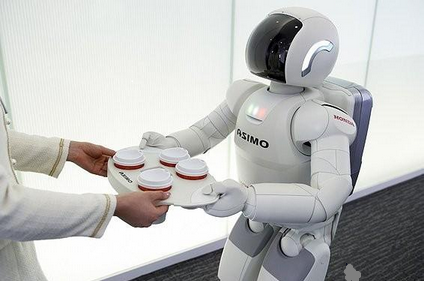
\includegraphics[width=10.00cm,height=5.10cm]{test.png}
     %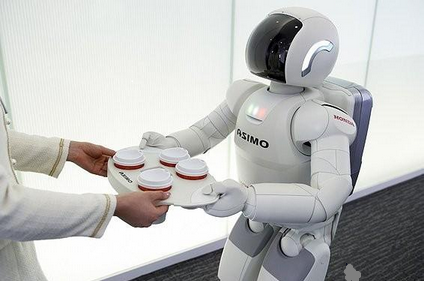
\includegraphics[width=0.5\linewidth]{test.png}
        \end{figure}
    \end{frame}

    \begin{frame}\frametitle{ttyUSB0}
        cd /etc/udev/rules.d/ \\
        touch serial-usb.rules\\
   %\begin{theorem}
%   KERNEL==\"ttyUSB0\",GROUP=\"uucp\",MODE=\"0666\"
   %\end{theorem}
    \end{frame}

    \begin{frame}\frametitle{挂载}
        sudo fdisk -l\\
        sudo mount -t nfts /dev/sda\quotes{n} /mnt/
    \end{frame}

    \begin{frame}\frametitle{change color}
        cd /usr/share/themes/Ambiance/gtk-3.0\\ %
        sudo vim gtk-main.css\\
        base\_color \#cce8cf\\
    \end{frame}

    \begin{frame}\frametitle{google change color}
        Google Chrome(谷歌浏览器)修改网页背景颜色的办法(比如修改为护眼的豆沙绿)  \\
        过客\\
    \end{frame}

  % \begin{frame}\frametitle{java}
  %   sudo vim etc/profile\\
  %   export JAVA\_HOME=/usr/bin/java/jdk1.8.0\_102\\
  %   export PATH=.:\$JAVA\_HOME/bin:\$PATH\\
  %   anaconda python\\
  % \end{frame}

  % \begin{frame}\frametitle{编译大型工程内存不足}
  %   error:\\
  %   g++:internal compiler error: Killed (program cc1plus)\\
  %   Please submit a full bug report,\\
  %   sudo mkswap /swapfile\\
  %   sudo swapon /swapfile\\
  %   编译完成后:\\
  %   sudo swapoff /swapfile\\
  %   sudo rm /swapfile\\
  % \end{frame}

    \begin{frame}\frametitle{Ubuntu to Mac}
        github FixLinux 
    \end{frame}

\end{CJK}

\end{document}

%%% Local Variables:
%%% mode: latex
%%% TeX-master: t
%%% End:
